\documentclass[tikz,border=2pt]{standalone}
\usepackage{amsmath,amssymb}
\usetikzlibrary{arrows.meta,decorations.pathreplacing}
\begin{document}
% One realized scenario at duration t: outgo Z_t + H_t = 100 + 5 = 105 against premium income Y_t = 80;
% the gross future loss is the excess L_t^g = 105 - 80 = 25 (positive: outgo exceeds income).
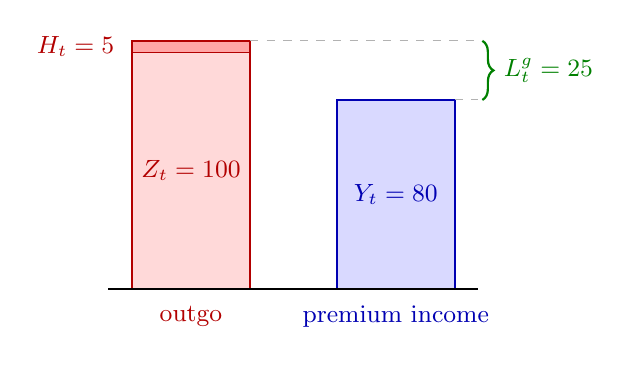
\begin{tikzpicture}[font=\small, >={Latex[length=2mm]}, y=0.03cm]
  \def\bw{1.5}
  % outgo bar
  \fill[red!15] (0,0) rectangle (\bw,100);
  \fill[red!35] (0,100) rectangle (\bw,105);
  \draw[red!70!black, thick] (0,0) rectangle (\bw,105);
  \draw[red!70!black, thin] (0,100) -- (\bw,100);
  \node[red!70!black] at (0.5*\bw,50) {$Z_t=100$};
  \node[red!70!black, anchor=east] at (-0.1,102.5) {$H_t=5$};
  % income bar
  \fill[blue!15] (2.6,0) rectangle (2.6+\bw,80);
  \draw[blue!70!black, thick] (2.6,0) rectangle (2.6+\bw,80);
  \node[blue!70!black] at (2.6+0.5*\bw,40) {$Y_t=80$};
  % loss gap
  \draw[gray!60, thin, dashed] (\bw,105) -- (2.6+\bw+0.3,105);
  \draw[gray!60, thin, dashed] (2.6+\bw,80) -- (2.6+\bw+0.3,80);
  \draw[green!50!black, thick, decorate, decoration={brace, amplitude=4pt}]
    (2.6+\bw+0.35,105) -- (2.6+\bw+0.35,80)
    node[midway, anchor=west, xshift=4pt] {$L_t^g=25$};
  % baseline and captions
  \draw[thick] (-0.3,0) -- (2.6+\bw+0.3,0);
  \node[red!70!black, anchor=north] at (0.5*\bw,-3) {outgo};
  \node[blue!70!black, anchor=north] at (2.6+0.5*\bw,-3) {premium income};
\end{tikzpicture}
\end{document}
